\documentclass[11pt]{article}

\usepackage{amssymb}
\usepackage{amsmath, esint}
\usepackage{amsthm}
\usepackage{array}
\usepackage{longtable}
\usepackage{mathtools}
\usepackage{pdfpages}
\usepackage{fancyhdr}
\usepackage[figurename=Figure]{caption}
\usepackage{empheq}
\usepackage{mdframed}
\usepackage[a4paper, left=1in,right=1in,top=1in,bottom=0.7in,footskip=0.6in,includeheadfoot]{geometry}
\usepackage{tikz}
\usepackage{pgfplots}
\usepackage{hyperref}
\usepackage{wrapfig}
\usepackage{enumitem}
\usepackage{lastpage}
\usepackage{zref-totpages}
\usepackage{float}

%title
\edef\mytitle{Precalculus}
\edef\mysubtitle{Lesson 6: Complex Numbers}
\edef\mydate{July 2, 2024}
\edef\myauthor{Tyler Wang}

\usetikzlibrary{calc, backgrounds,angles, quotes}
\usepgfplotslibrary{polar}

\tikzset{
    partial ellipse/.style args={#1:#2:#3}{
        insert path={+ (#1:#3) arc (#1:#2:#3)}
    }
}

\setlength{\parskip}{10pt}
\setlength{\parindent}{0pt}

\fancyhf{}
\fancyfoot[l]{\copyright \,\,\myauthor}
\fancyhead[L]{\mysubtitle}
\fancyhead[r]{\mytitle}
\fancyfoot[c]{Page \thepage \hspace{1pt} of \ztotpages}
\pagestyle{fancy}

\fancypagestyle{plain}{
\fancyhf{}
\fancyfoot[l]{\copyright \,\,\myauthor}
\fancyfoot[c]{Page \thepage \hspace{1pt} of \ztotpages}
\renewcommand{\headrulewidth}{0pt}}

\newmdtheoremenv{lemma}{Lemma}
\newmdtheoremenv{prop}{Proposition}
\newmdtheoremenv{define}{Definition}
\newmdtheoremenv{theorem}{Theorem}
\newmdtheoremenv{cor}{Corollary}

\numberwithin{lemma}{section}
\numberwithin{equation}{section}
\numberwithin{define}{section}
\numberwithin{prop}{section}
\numberwithin{figure}{section}
\numberwithin{theorem}{section}
\numberwithin{cor}{section}

\newcounter{ex}[section]
\newenvironment{ex}[0]{

	\refstepcounter{ex}
    \subsection*{Example \theex .}
    }
    {
    \hfill$\spadesuit$
    \par
    }
\numberwithin{ex}{section}

\def\real{\mathbb{R}}
\def\complex{\mathbb{C}}
\def\rat{\mathbb{Q}}
\def\nat{\mathbb{N}}
\def\integ{\mathbb{Z}}
\def\mod#1{\mathbb{Z}_{#1}}
\def\cpx{\mathbb{C}}

\def\paren#1{\left(#1\right)}
\def\sbrak#1{\left[#1\right]}
\def\cbrak#1{\left\{#1\right\}}

\def\ceil#1{\left\lceil #1 \right\rceil}
\def\floor#1{\left\lfloor #1 \right\rfloor}
\def\abs#1{\left\lvert #1 \right\rvert}
\def\abrak#1{\left\langle #1 \right\rangle}
\def\bra#1{\left\langle #1 \right\rvert}
\def\ket#1{\left\lvert #1 \right\rangle}
\def\braket#1#2{\left\langle #1 \left.\right\lvert #2 \right\rangle}

\def\jand{\quad\text{and}\quad}
\def\jor{\quad\text{or}\quad}
\def\for{\quad\text{for }\,}

\def\ieval#1#2{\Bigg|^{#2}_{#1}}
\def\deval#1{\bigg|_{#1}}

\def\diff#1#2{\frac{d#1}{d#2}}
\def\pdiff#1#2{\frac{\partial#1}{\partial#2}}

\def\sec#1{\section*{#1}\addtocounter{section}{1}\setcounter{subsection}{0}}

\hypersetup{
    colorlinks=true,
    urlcolor=blue,
    linkcolor=magenta,
    pdfborderstyle={/S/U/W 1}
}

\setlength\extrarowheight{3pt}

\title{\mytitle \\ [2ex] \Large \mysubtitle}
\date{\small Modified \mydate}
\author {Tyler Wang\thanks{
\href{mailto:wangtyler123@gmail.com}{wangtyler123@gmail.com}}}

\begin{document}
\maketitle
\section{Polor Coordinates}
\subsection{Polar Plane}
In this section, I'm going to try to introduce to you a new way of plotting. 
Throughout your entire math career thus far, you may have only been exposed to one type of coordinate system, the cartesian plane.
But here, we are going to explore ways we can plot things on a graph that don't have an $x$ or a $y$ coordinate.

\begin{figure}[h]
\centering
	\resizebox{0.5\textwidth}{!}{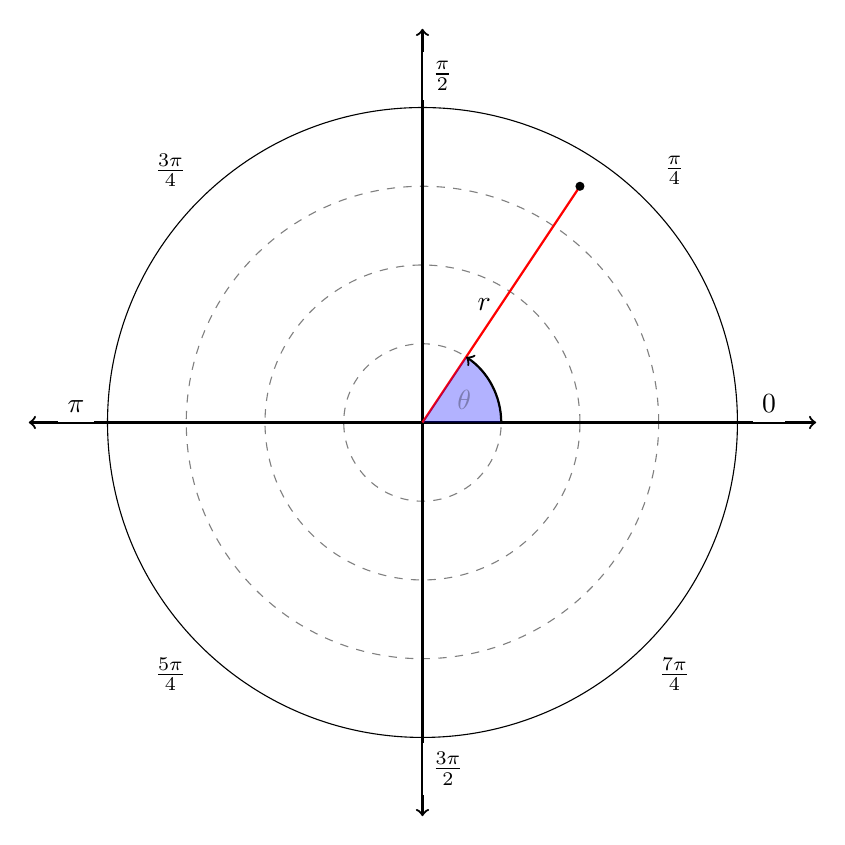
\begin{tikzpicture}
		\coordinate (O) at (0,0);

		\draw[gray, thin, dashed] (O) circle (1);
		\draw[gray, thin, dashed] (O) circle (2);
		\draw[gray, thin, dashed] (O) circle (3);
		\draw (O) circle (4);
		
		\draw[thick, <->] (-5,0) -- (5,0) coordinate (P);
		\draw[thick, <->] (0,-5) -- (0, 5);
		
		\node[above, fill=white] (a) at (4.4,0) {$0$};
		\node[right, fill=white] (b) at (0,4.4) {$\frac{\pi}{2}$};
		\node[above, fill=white] (c) at (-4.4,0) {$\pi$};
		\node[right, fill=white] (d) at (0,-4.4) {$\frac{3\pi}{2}$};
		
		\node[fill=white] (e) at (3.2,3.2) {$\frac{\pi}{4}$};
		\node[fill=white] (f) at (-3.2,3.2) {$\frac{3\pi}{4}$};
		\node[fill=white] (g) at (-3.2,-3.2) {$\frac{5\pi}{4}$};
		\node[fill=white] (h) at (3.2,-3.2) {$\frac{7\pi}{4}$};
		
		\draw[red,thick] (O) -- (2,3) node[midway, black, left] {$r$};
		\filldraw (2,3) coordinate (A) circle (0.05);
		\pic["$\theta$", draw, ->, black, thick, fill=blue, fill opacity=0.3, angle radius=1cm] {angle = P--O--A};
	\end{tikzpicture}}
	\caption{}
	\label{fig:polar-intro}
\end{figure}

First, let's define polar coordinates. Like cartesian coordinates, a polar coordinate is also written as an ordered pair, except with the variables $r$ and $\theta$, where $r$ is the distance from the \textbf{pole}, or origin, and $\theta$ is the angle that a ray connecting the pole and point makes with the polar axis, as seen in figure \eqref{fig:polar-intro}.
Normally we set the polar axis as the positive $x$ axis and let positive angles open counterclockwise.
Since an angle of $2\pi$ is congruent to an angle of $0$, the consequence of using an angle to label a point is that there are infinitely many ordered pairs that we can use to represent a position. 
For this reason, we typically restrict $\theta\in(-\pi,\pi]$. The choice we make here is arbitrary, so we could have chosen any interval we'd like, so long as every angle on the plane is reached.
But even still, there are still multiple choices of ordered pairs that would label the point.
Let's illustrate this fact in this next example.

\begin{ex}
	For this example, let's find all the possible ways we can label the point $\paren{2,\frac{\pi}{3}}$ given $\theta\in(-\pi,\pi]$.
	First, I've plotted this point in figure \eqref{fig:plot-point}.
	\begin{figure*}[h]
	\centering
	\resizebox{0.5\textwidth}{!}{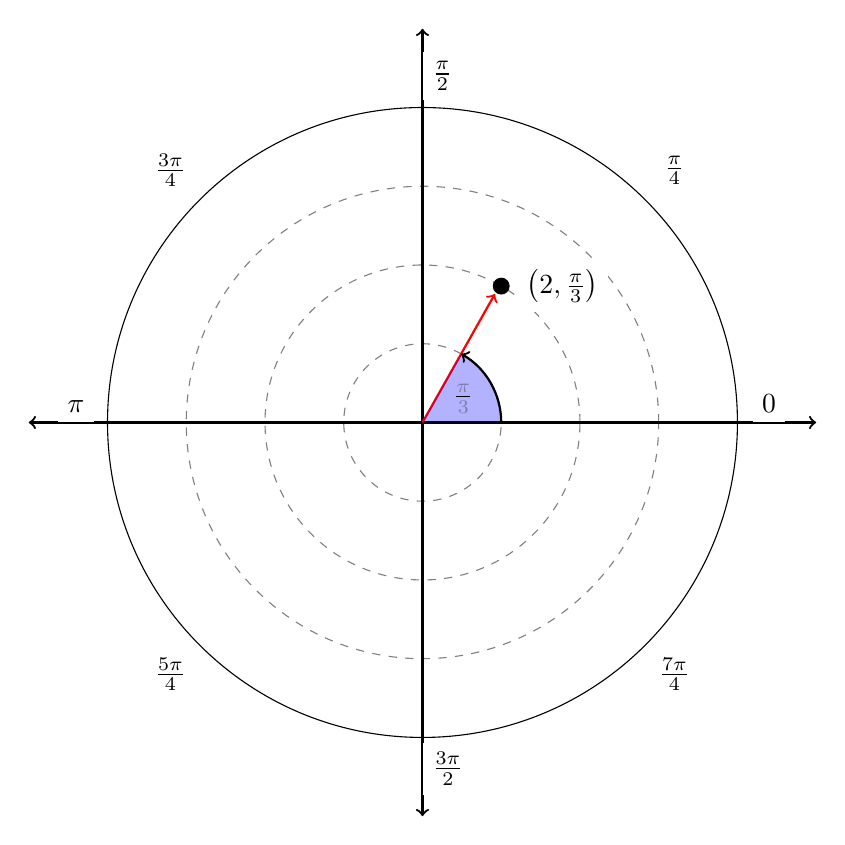
\begin{tikzpicture}
		\coordinate (O) at (0,0);

		\draw[gray, thin, dashed] (O) circle (1);
		\draw[gray, thin, dashed] (O) circle (2);
		\draw[gray, thin, dashed] (O) circle (3);
		\draw (O) circle (4);
		
		\draw[thick, <->] (-5,0) -- (5,0) coordinate (P);
		\draw[thick, <->] (0,-5) -- (0, 5);
		
		\node[above, fill=white] (a) at (4.4,0) {$0$};
		\node[right, fill=white] (b) at (0,4.4) {$\frac{\pi}{2}$};
		\node[above, fill=white] (c) at (-4.4,0) {$\pi$};
		\node[right, fill=white] (d) at (0,-4.4) {$\frac{3\pi}{2}$};
		
		\node[fill=white] (e) at (3.2,3.2) {$\frac{\pi}{4}$};
		\node[fill=white] (f) at (-3.2,3.2) {$\frac{3\pi}{4}$};
		\node[fill=white] (g) at (-3.2,-3.2) {$\frac{5\pi}{4}$};
		\node[fill=white] (h) at (3.2,-3.2) {$\frac{7\pi}{4}$};
		
		\filldraw (1,1.732) circle (0.1) node[right, fill=white, xshift=0.2cm] {$\paren{2,\frac{\pi}{3}}$};
		\draw[->,red,thick] (O) -- (0.92,1.632) coordinate (A);
		\pic["$\frac{\pi}{3}$", draw, ->, black, thick, fill=blue, fill opacity=0.3, angle radius=1cm] {angle = P--O--A};
	\end{tikzpicture}}
	\caption{}
	\label{fig:plot-point}
	\end{figure*}
	Because of the way, we defined $\theta$, we go around the circle once, so with a radius of $2$, $\frac{\pi}{2}$ is the only time we hit our desired point. 
	But since there aren't any restrictions on $r$, we can allow $r$ to be negative. What this would mean is that instead of moving in the direction of the ray defined by the angle, we would go in the opposite direction.
	\begin{figure*}[h]
	\centering
	\resizebox{0.5\textwidth}{!}{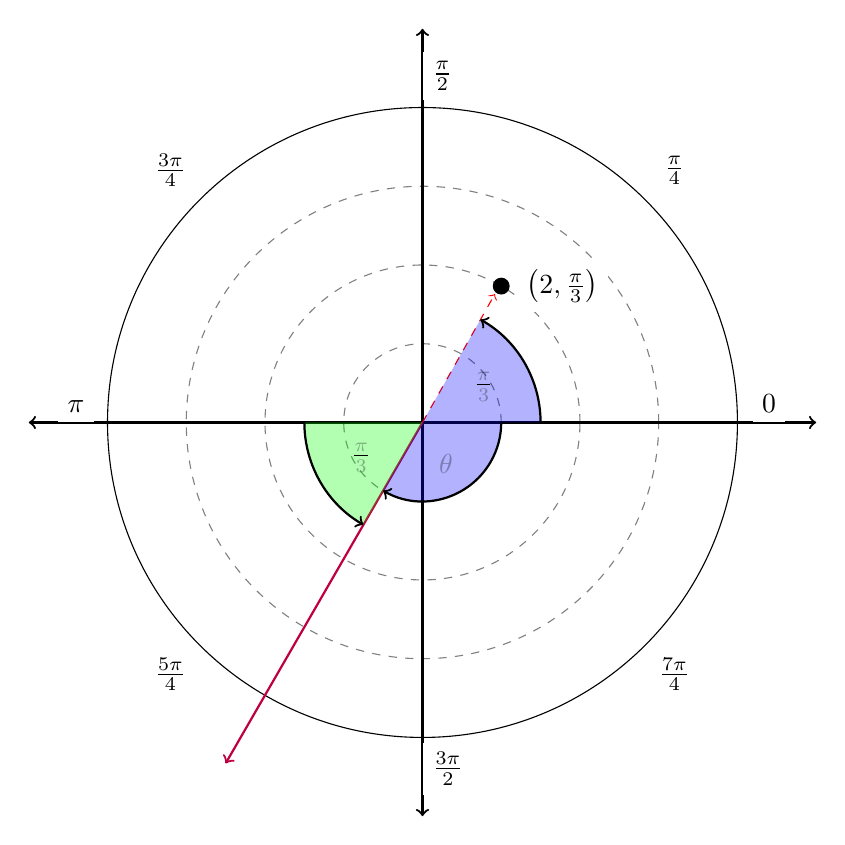
\begin{tikzpicture}
		\coordinate (O) at (0,0);
		\coordinate (B) at (0.92,1.632);

		\draw[gray, thin, dashed] (O) circle (1);
		\draw[gray, thin, dashed] (O) circle (2);
		\draw[gray, thin, dashed] (O) circle (3);
		\draw (O) circle (4);
		
		\draw[thick, <->] (-5,0) coordinate (Q) -- (5,0) coordinate (P);
		\draw[thick, <->] (0,-5) -- (0, 5);
		
		\node[above, fill=white] (a) at (4.4,0) {$0$};
		\node[right, fill=white] (b) at (0,4.4) {$\frac{\pi}{2}$};
		\node[above, fill=white] (c) at (-4.4,0) {$\pi$};
		\node[right, fill=white] (d) at (0,-4.4) {$\frac{3\pi}{2}$};
		
		\node[fill=white] (e) at (3.2,3.2) {$\frac{\pi}{4}$};
		\node[fill=white] (f) at (-3.2,3.2) {$\frac{3\pi}{4}$};
		\node[fill=white] (g) at (-3.2,-3.2) {$\frac{5\pi}{4}$};
		\node[fill=white] (h) at (3.2,-3.2) {$\frac{7\pi}{4}$};
		
		\filldraw (1,1.732) circle (0.1) node[right, fill=white, xshift=0.2cm] {$\paren{2,\frac{\pi}{3}}$};
		\draw[->,purple, thick] (O) -- (-2.5,-4.330) coordinate (A);
		\draw[->,red,dashed] (O) -- (0.92,1.632);
		\pic["$\theta$", draw, <-, black, thick, fill=blue, fill opacity=0.3, angle radius=1cm] {angle = A--O--P};
		\pic["$\frac{\pi}{3}$", draw, ->, black, thick, fill=green, fill opacity=0.3, angle radius=1.5cm] {angle = Q--O--A};
		\pic["$\frac{\pi}{3}$", draw, ->, black, thick, fill=blue, fill opacity=0.3, angle radius=1.5cm] {angle = P--O--B};
	\end{tikzpicture}}
	\caption{}
	\label{fig:re-plot-point}
	\end{figure*}
	As in figure \eqref{fig:re-plot-point}, if we draw a ray opposite of our original ray, and use that angle, we can use that angle to label our point. In this case, we notice the angle of our new ray with the $-x$-axis is $\frac{\pi}{3}$, since the red line and $x$-axis form vertical angles, by doing a bit of geometry, we find our angle is $-\frac{2\pi}{3}$, hence the other way we can label this point is
	$$(-2,\frac{2\pi}{3}).$$
\end{ex}

\subsection{Converting Between Polar and Cartesian}
As you might have already suspected, all of this polar stuff is reminiscent of how trig functions. We can leverage trig to convert between cartesian coordinates and polar.

\begin{theorem}
Let $(r,\theta)$ be a point in polar coordinates, then the corresponding point in cartesian coordinates can be given as
$$(r\cos(\theta),r\sin(\theta))$$
\label{thm:poletocart}
\end{theorem}
This theorem comes directly from the definition of $\cos(x)$ and $\sin(x)$ by multiplying the circle by a factor of $r$. Using this, we can now try to convert equations plotted in polar, into equations we can plot in Cartesian or the other way around.

\begin{ex}
	Let's convert $r=2\sin\theta$ to cartesian to identify the shape of this curve.
	Multiplying $r$ on both sides gives
	$$r^2=2r\sin\theta.$$
	The utility of this operation might not be immediately clear, but since we know
	$$x=r\cos\theta \jand y=r\sin\theta$$
	having that extra $r$ term allows us to substitute out the $r\sin\theta$ term fo $y$. Therefore
	$$r^2=2y$$
	Since we know $r$ is simply the distance to the origin, using Pythagorean's theorem,
	$$r=\sqrt{x^2+y^2}$$
	therefore our equation becomes
	$$x^2+y^2=2y$$
	Then rearranging the equation and completing the square allows us to get
	$$x^2+y^2-2y=0$$
	$$x^2+y^2-2y+1=1$$
	$$x^2+(y-1)^2=1$$
	which we see this equation simply represents a circle centered at $(0,1)$.
\end{ex}

\begin{ex}
	In this example, let's find the corresponding cartesian form of the equation
	$$r=\frac{6}{\cos\theta+3\sin\theta}.$$
	Since the trig functions in the denominator lack the factor of $r$ that allows us to easily substitute them for $x$ and $y$, we can divide both sides by $r$ to allow for this.\footnote{Since the only way for $r$ to be 0 is if the numerator is 0, we know this is not possible since the numerator is a non-zero constant.}
	Therefore
	$$1=\frac{6}{r\cos\theta+3r\sin\theta}$$
	$$1=\frac{6}{x+3y}$$
	$$x+3y=6$$
	hence we conclude this is a line with a slope of $-\frac{1}{3}$ with a $y$-intercept of $2$.
\end{ex}

\section{Complex Numbers}
\subsection{Polar Form}
Similar to coordinates in a plane, complex numbers also have a corresponding polar form. But before we examine that, we must define an operation that will be key for defining polar complex numbers.

I've mentioned that the complex numbers are not an ordered set, but similar to the real numbers, complex numbers have this notion of distance. To describe the distance, we define the following:
\begin{define}
	Let the absolute value, (modulus) be defined as
	$$|z|=\sqrt{z\bar{z}}$$
\end{define}
Since we know that $z\bar{z}$ is always positive, from a previous lesson, so this value will always be positive. 
This definition, in reality, is arbitrary, there are many other ways we could have chosen to define this, as long as they satisfy a certain set of criteria. But we chose this definition since it allows our complex plane to be a plane and agrees with our other definitions of distance in a plane.

Now we have a method of finding the distance from any complex number to the origin, we also need an operation that measures the angle a complex number makes with the positive real axis.
\begin{define}
	Let $\arg: \complex \to \real$ be defined as a multivalued function where $\arg(z)$ returns the argument (angle with respect to the positive real axis) of $z$.
\end{define}

We technically could've used $\tan^{-1}\paren{\frac{b}{a}}$, but due to this only being defined for $\sbrak{-\frac{\pi}{2},\frac{\pi}{2}}$, this is no good for numbers that are in the second or third quadrant. So in complex analysis, we generalize this operation with $\arg(z)$. Now notice this is a \textbf{multivalued} function, so this is not a function that we defined in Lesson 2. Instead, for any given complex number, it outputs an infinite number of angles.\footnote{
This makes sense since as we talked about, if $\theta\in\real$, then there are an infinite number of ways to label an angle.}
For this reason, we typically restrict the function to only output on the interval $(-\pi,\pi]$. We call this the \textbf{principle argument} and typically denote this function as $\text{Arg}(z)$.

Now we can define polar complex numbers. Since we know we can label a complex number in polar form with the ordered pair $(|z|,\text{Arg}(z))$, using theorem \eqref{thm:poletocart},
$$z=|z|(\cos(\text{Arg}(z))+i\sin(\text{Arg}(z)))$$
Sometimes we shorthand this notation and simply write
$$z=|z|\text{cis}(\text{Arg}(z))$$
where
$$\text{cis}(\theta)=\cos(\theta)+i\sin(\theta)$$

\begin{ex}
	In this example, I'd like to show you how to multiply a complex number in polar form. We know the general form of a complex number in polar form is
	$$z_1=r_1\text{cis}(\theta_1)$$
	$$z_2=r_2\text{cis}(\theta_2)$$
	where
	$$r_1=|z_1| \jand \theta_1=\text{Arg}(z_1)$$
	$$r_2=|z_2| \jand \theta_2=\text{Arg}(z_2)$$
	Then
	$$z_1z_2=(r_1\text{cis}(\theta_1)) \cdot (r_2\text{cis}(\theta_2))$$
	$$=r_1r_2(\cos(\theta_1)+i\sin(\theta_1))(\cos(\theta_2)+i\sin(\theta_2))$$
	$$=r_1r_2(\cos(\theta_1)\cos(\theta_2)-\sin(\theta_1)\sin(\theta_1)+i\cos(\theta_1)\sin(\theta_2)+i\sin(\theta_1)\cos(\theta_2))$$
	Then using the cosine and sine sum identities,
	$$=r_1r_2(\cos(\theta_1+\theta_2)+i\sin(\theta_1+\theta_2))$$
	$$=r_1r_2\text{cis}(\theta_1+\theta_2)$$
\end{ex}

 As you can see in the last example, $\text{cis}(\theta)$ sort of acts like an exponential, in the sense that multiplying them together will add its arguments. The reason for this is that it turns out $\text{cis}(x)$ is just how we can define the complex exponential.
 
 \begin{theorem}[Euler's Theorem]
 	Let $\theta\in\real$, then
 	$$e^{i\theta}=\cos(\theta)+i\sin(\theta)$$	
 \end{theorem}
 \begin{proof}
 	Postponed indefinitely.
 \end{proof}
 
 Now, we see, we can write the polar form of a complex number as
 $$z=|z|e^{i\arg(z)}.$$
Now with this, we can use the properties that we defined for exponentials to perform complex multiplication and division.

\begin{theorem}
	If $z\in\complex$, then 
	$$\bar{z}=|z|e^{-i\arg(z)}$$
\end{theorem}
\begin{proof}
	Let $r=|z|$ and $\theta=\arg(z)$, where $\theta$ is any choice of $\arg(z)$.
	Then
	$$z=re^{i\theta}=r(\cos(\theta)+i\sin(\theta))$$
	For $\bar{z}$,
	$$\bar{z}=r(\cos(\theta)-i\sin(\theta))$$
	Then using the odd and even properties of trig functions:
	$$\bar{z}=r(\cos(-\theta)+i\sin(-\theta)$$
	$$=re^{-i\theta}$$
\end{proof}

\subsection{Roots of Numbers}
Now using complex exponentials, let's define root operations in terms of complex numbers. As I've stated before, taking a root in complex numbers will result in multiple outputs, no matter if the power is odd or even. Let's find out how to compute these roots in general.

\begin{ex}
	Let's compute in general the $n$th root of $z$. We know for $r,\theta$,
	$$z=re^{i\theta}$$
	Therefore taking the $n$th root gives
	$$\sqrt[n]{z}=(z)^{\frac{1}{n}}=r^{\frac{1}{n}}(e^{i\theta})^\frac{1}{n}
	=r^{\frac{1}{n}}\exp\paren{\frac{i\theta}{n}}$$
	Since angles $2\pi$ apart are congruent,
	$$=r^{\frac{1}{n}}\exp\paren{\frac{i\theta+2i\pi k}{n}} \for k\in\integ.$$
	Then taking only the positive result from $r^{\frac{1}{n}}$\footnote{Because turns out the others are redundant.}
	and setting $s=r^\frac{1}{n}$
	$$=s\exp\paren{\frac{i\theta}{n}+\frac{2i\pi k}{n}}$$
	Notice here, that although we defined $k\in\integ$, it turns out equivilently, we could have just defined $k\in\{0,1,...,n-1\}$, since any other $k\in\integ$ would just produce overlapping angles and would be redundant.
\end{ex}

\begin{ex}
	With the formula we computed before, let's compute the cube root of $z=1+i$.
	First, we compute the modulus of $z$:
	$$|z|=\sqrt{(1+i)(1-i)}=\sqrt{2}$$
	Then for the principle argument:
	$$\text{Arg}(z)=\tan^{-1}(1)=\frac{\pi}{4}\footnotemark$$
	\footnotetext{Of course we check that $tan^{-1}(x)$ output in the right quadrant, or we would need to modify the output.}
	Therefore
	$$z=\sqrt{2}\exp\paren{\frac{i\pi}{4}}$$
	Then using the formula in the last example:
	$$\sqrt[3]{z}=\sqrt[6]{2}\exp\paren{\frac{i\pi}{4}\cdot\frac{1}{3}+\frac{2i\pi k}{3}} \for k\in\integ$$
	$$=\sqrt[6]{2}\exp\paren{\frac{i\pi}{12}+\frac{2}{3}i\pi k}.$$
	Then, the 3 unique solutions are
	$$\cbrak{\sqrt[6]{2}\exp\paren{\frac{i\pi}{12}},\sqrt[6]{2}\exp\paren{\frac{3i\pi}{4}},\sqrt[6]{2}\exp\paren{\frac{17i\pi}{12}}}$$
\end{ex}
\subsection{Complex Logarithms}
\begin{ex}
	In this example, I'm going to compute a complex logarithm in general. In terms of notation, we typically use $\ln(x)$ to define a complex natural logarithm, and in the context of complex numbers, we use $\log(z)$ to denote a complex natural logarithm.\footnote{We generally don't talk about logarithms for complex variables with arbitrary bases, since turns out, those are generally less useful, and can be replaced simply by dividing by the respective base.}
	Thus since $z=re^{\i\theta}$, by using the definition of the logarithm and its properties:
	$$\log(z)=\log(re^{\i\theta})=\ln(r)+\log(e^{\i\theta})=\ln(r)+i\theta.$$
	Since 
	$$\theta\cong\theta +2\pi k \for k\in\integ,$$
	it turns out $\log(z)$ is a multivalued functions outputting
	$$\log(z)=\ln(r)+i\theta+2i\pi k.$$
	More generally,
	$$=\ln(r)+i\arg(z)$$
	or if taking the principle value:
	$$\text{Log}(z)=\ln(r)+i\text{Arg}(z)$$
\end{ex}
\begin{ex}
	Now using the above formula, let's compute $\text{Log}(-\sqrt{3}+i)$.
	First finding the modulus of $z$ we get
	$$|z|=\sqrt{z\bar{z}}=\sqrt{(-\sqrt{3}+i)(-\sqrt{3}-i)}=2$$
	Then computing the principle argument:
	$$\text{Arg}(z)=\tan^{-1}\paren{-\frac{1}{\sqrt{3}}}=\frac{5\pi}{6}\footnotemark$$
	\footnotetext{Make sure we chose the domain for $\tan^{-1}(\theta)$ that outputs in the right quadrant, don't just plug this into a calculator.}
	Therefore,
	$$\text{Log}(z)=\ln(2)+\frac{5i\pi}{6}$$
	or if we expand to all outputs of $\log(z)$,
	$$\log(z)=\ln(2)+\frac{5i\pi}{6}+2i\pi k \for k\in\integ$$
	
\end{ex}
\end{document}









